\section{Experiment results}
The authors retrain the model with a different dataset to solve the Upper Body Detection problem. The dataset contains 98 images of people or groups of people. The authors concern 4 types of upper body, which is used as 4 classes for the ground truth.\\
The 4 types of upper body are: face\_wide, face\_side, upper\_body\_wide (ub\_wide), upper\_body\_side (ub\_side)
The number of images that each class appears in is as the table below:

\begin{center}
	\begin{tabular}{|c|c|c|c|}
		\hline
		\textbf{face\_wide} & \textbf{face\_side} & \textbf{upper\_body\_wide} & \textbf{upper\_body\_side}\\ 
		\hline
		51 & 43 & 31 & 62 \\
		\hline
	\end{tabular}
\end{center}

To rate the result, we recommend a new scale:\\
Let R = \((C - W) / A\)

Where:\\
R (rating) is the rating of the detection algorithm on a specific test. We want to maximize this value. And we can use this value to tell if one algorithm is better than another.\\
C (correct) is the number of correct objects (upper body or face) detected.\\
W (wrong) is the number of objects that is mistakenly detected.\\
A (all) is the total number of faces and upper bodies appeared in the images used for testing.\\

Let see why this formula works. We want to maximize C to reach A (the total number of objects in the test). Thus, \(C / A\) is pretty much the right formula for this detection problem. It represents the posibility that an object will be detected. The higher this value is, the better our algorithm is. But we don't want to forget that sometimes our detection system fails to detect an object and claims one object to be another. So we add the W value to the formula. In that way even the algorithm manages to detect all the objects in the test, but meanwhile mistake other objects to be faces or upper bodies, it still gets a bad rating. 

The authors run the model on 5 tests. Each test contains 10 images. After that, we calculate the R values for each test and calculate the average value avg(R).

The results can be desmonstrated by the following images:
%\begin{figure}
%	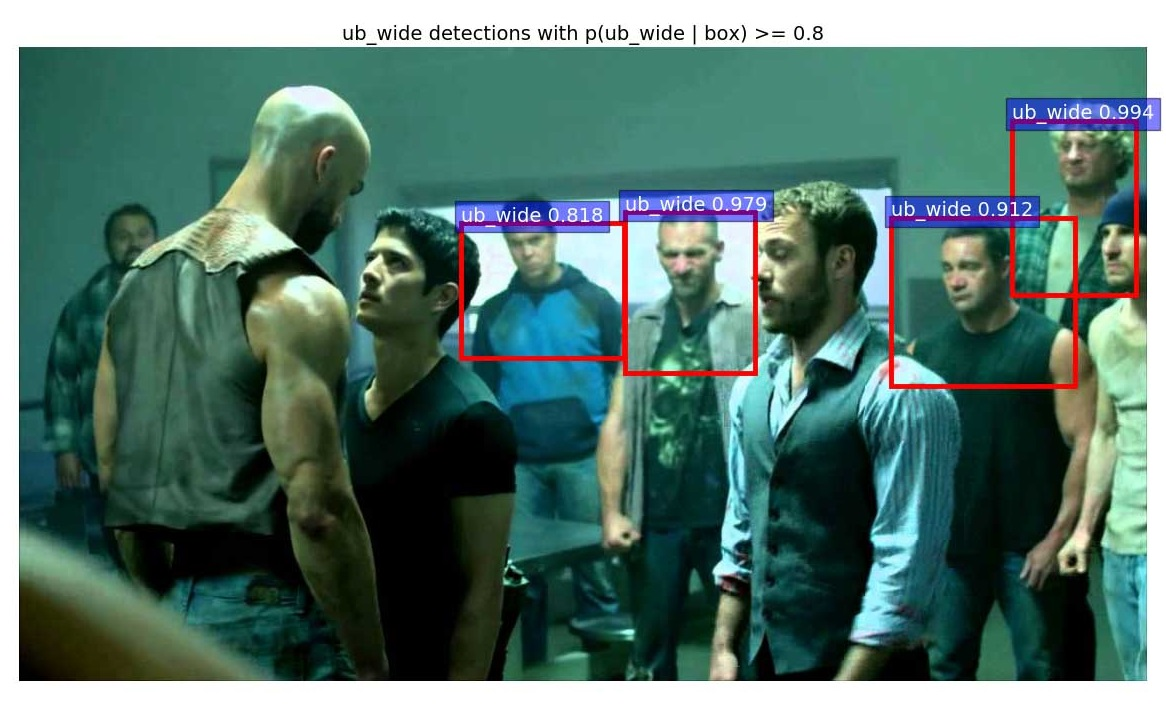
\includegraphics[width=0.7\linewidth]{img1}
%	\caption{}
%	\label{fig:res1}
%\end{figure}
\begin{figure*}[h]
	\centering
	\begin{subfigure}[b]{0.3\textwidth}
		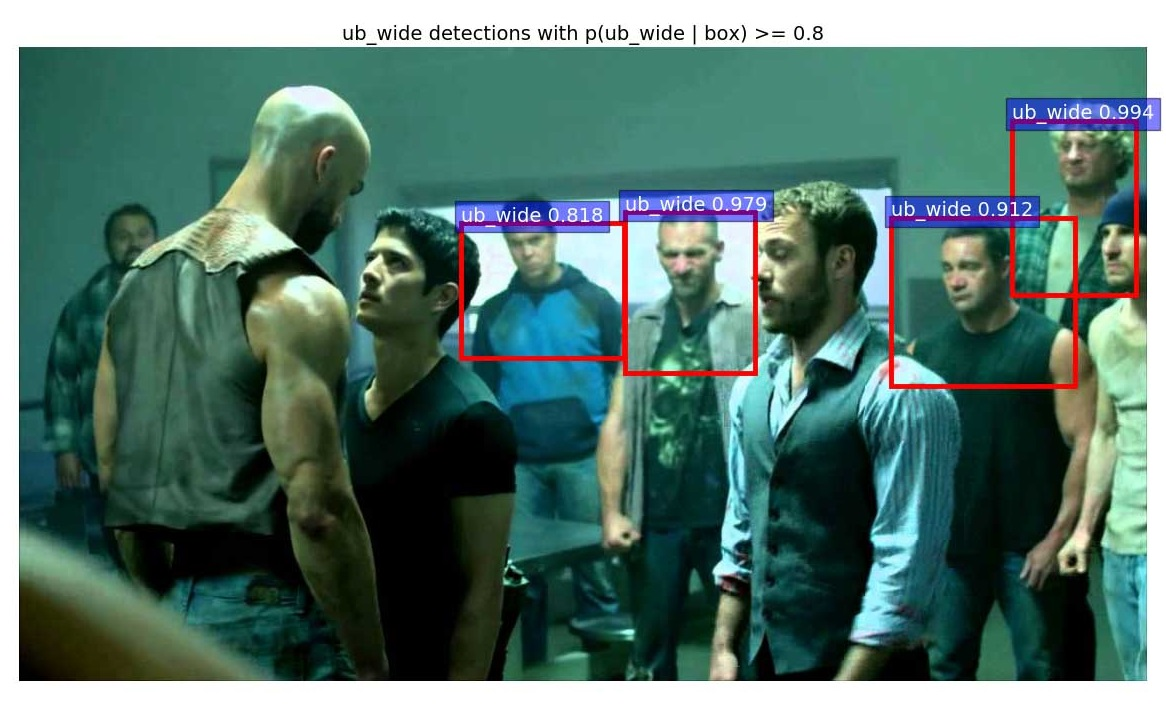
\includegraphics[width=\textwidth]{img1}
		\caption{}
		\label{fig:res1}
	\end{subfigure}
	~
	\begin{subfigure}[b]{0.3\textwidth}
		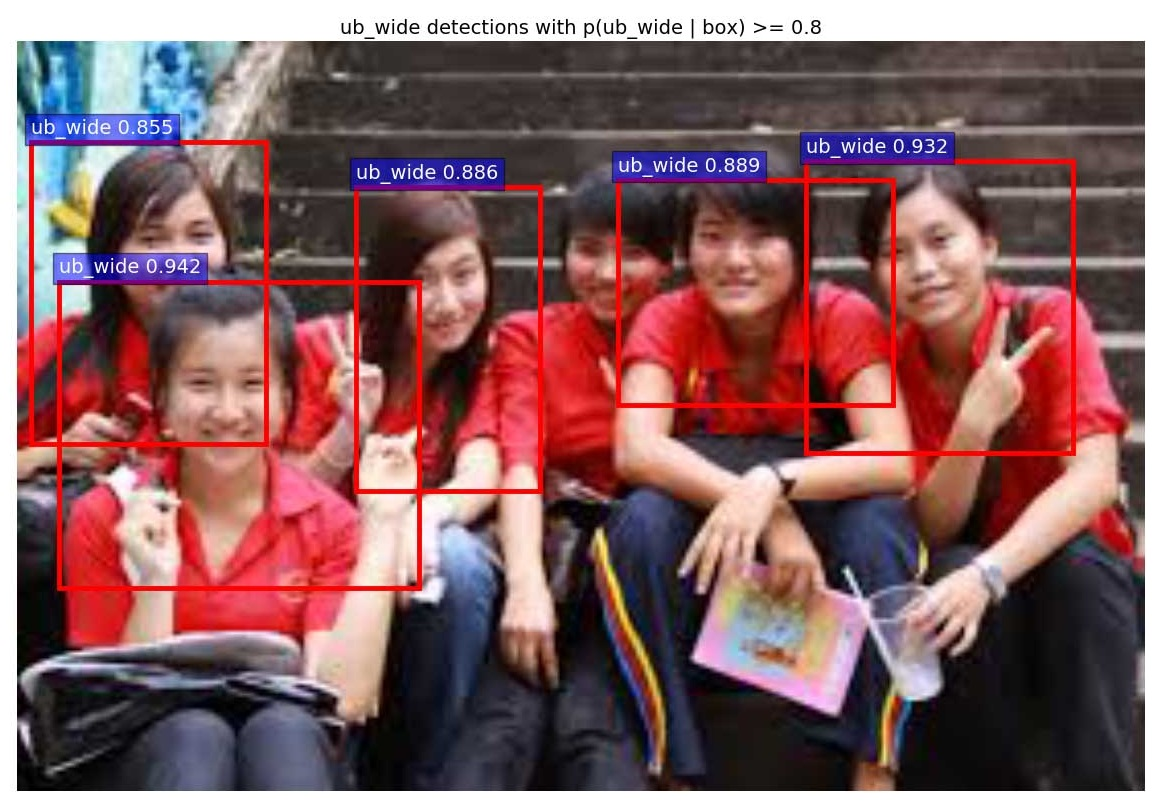
\includegraphics[width=\textwidth]{img2}
		\caption{}
		\label{fig:res2}
	\end{subfigure}
	~ %add desired spacing between images, e. g. ~, \quad, \qquad, \hfill etc. 
	%(or a blank line to force the subfigure onto a new line)
	\begin{subfigure}[b]{0.3\textwidth}
		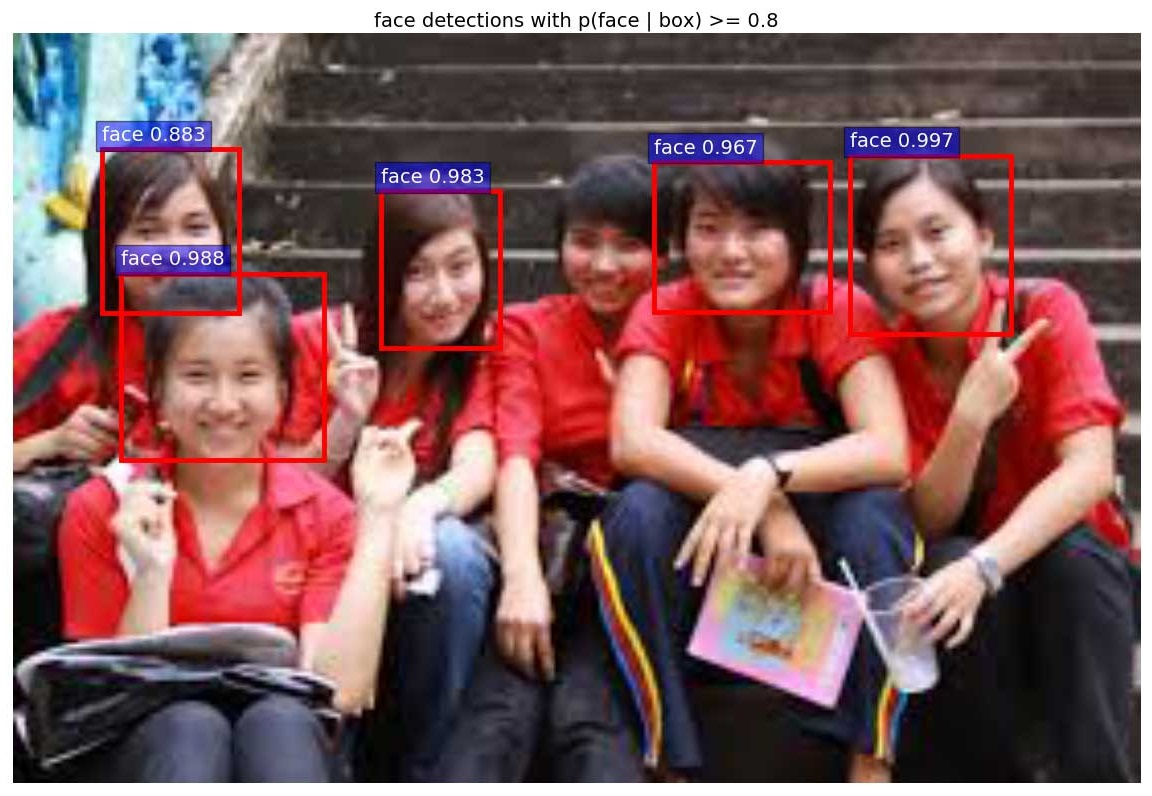
\includegraphics[width=\textwidth]{img3}
		\caption{}
		\label{fig:res3}
	\end{subfigure}
	~ %add desired spacing between images, e. g. ~, \quad, \qquad, \hfill etc. 
	%(or a blank line to force the subfigure onto a new line)
	\begin{subfigure}[b]{0.3\textwidth}
		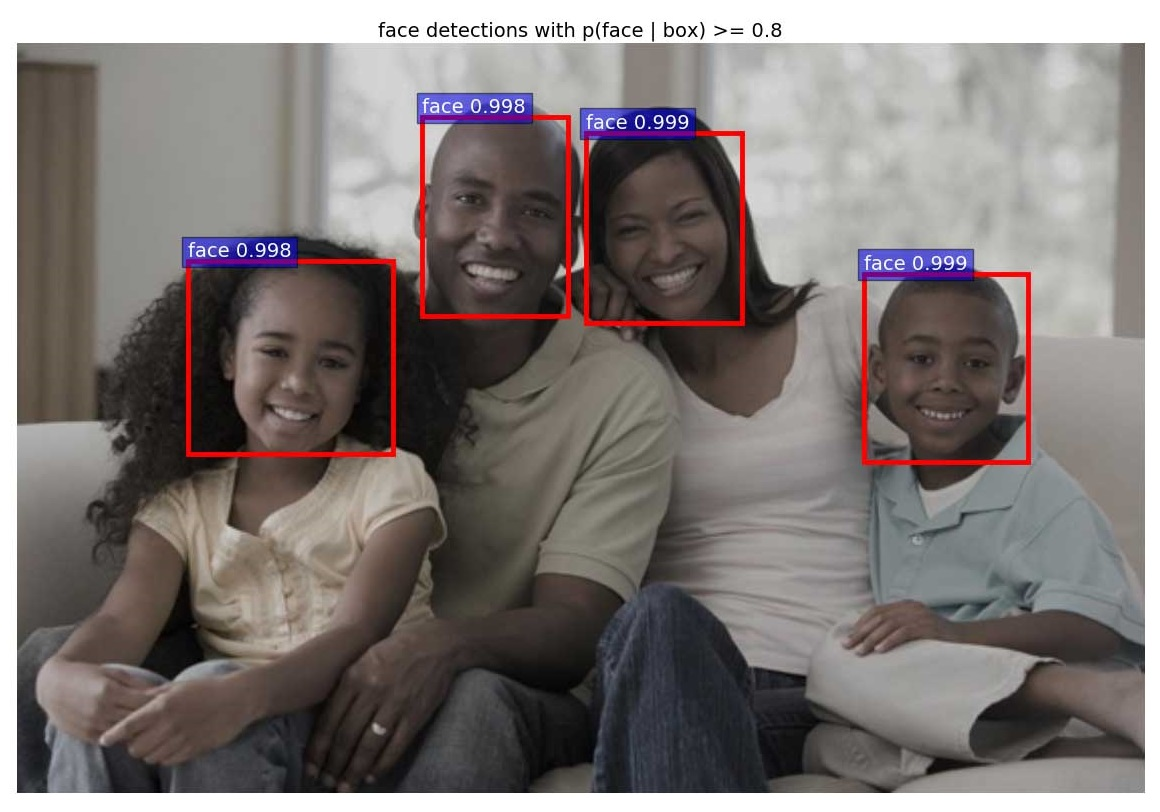
\includegraphics[width=\textwidth]{img4}
		\caption{}
		\label{fig:res4}
	\end{subfigure}
	~
	\begin{subfigure}[b]{0.3\textwidth}
		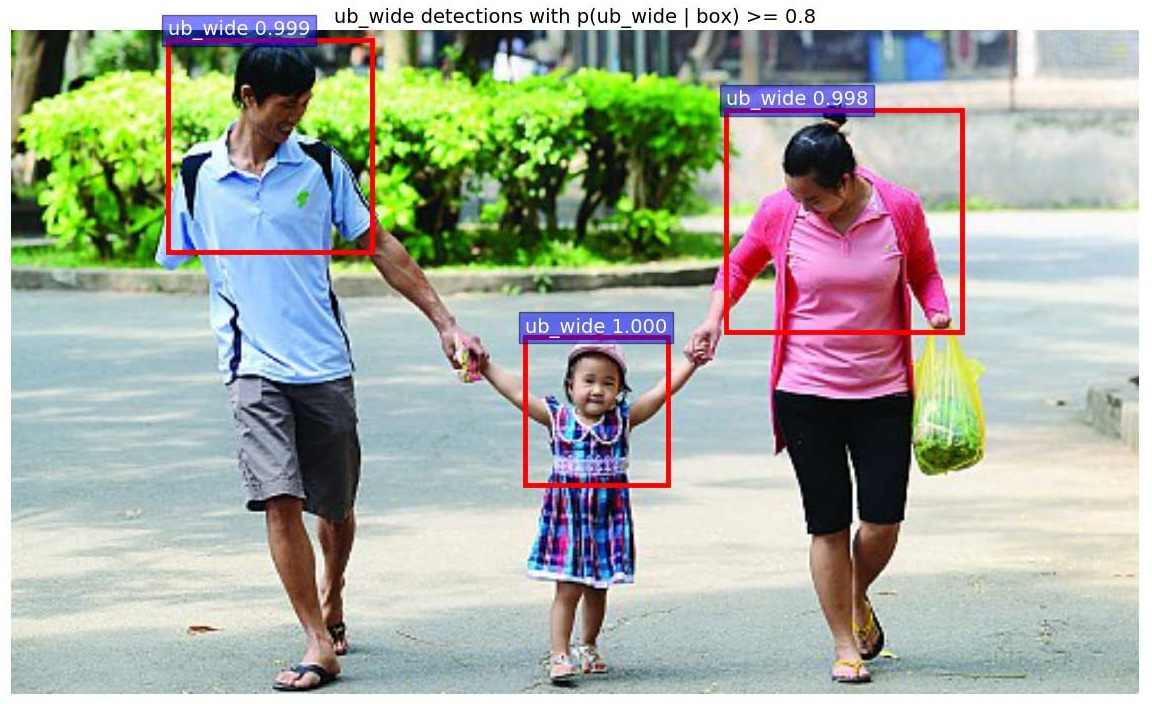
\includegraphics[width=\textwidth]{img5}
		\caption{}
		\label{fig:res5}
	\end{subfigure}
	~
	\begin{subfigure}[b]{0.3\textwidth}
		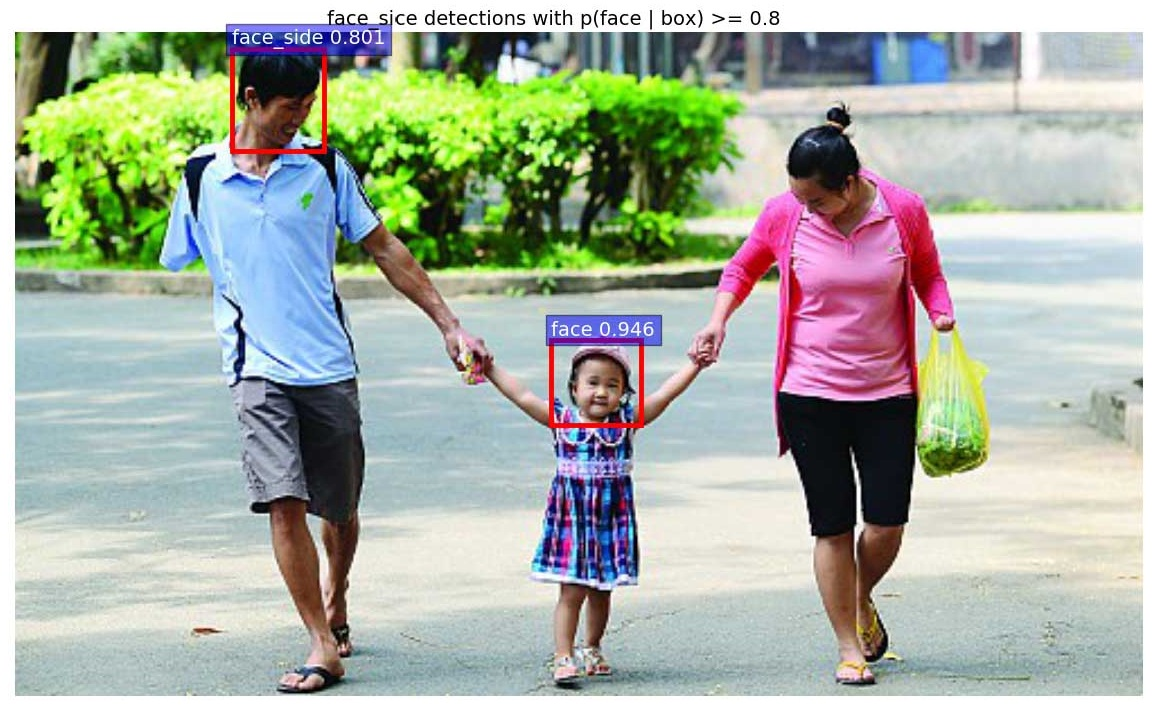
\includegraphics[width=\textwidth]{img6}
		\caption{}
		\label{fig:res6}
	\end{subfigure}
	\caption{Result pictures}\label{fig:animals}
\end{figure*}

And here we see in figure \ref{fig:res1}, most men's upper bodies are detected, except for 2 men on the left and 1 man on the right. This is because these upper bodies are not regular and the angles of their body are not included in the training set. 

In this case, R = 4/9 ( \(<50\) \%), 4 upper bodies are detected among 9 upper bodies.
this is still an encouraging result considering the complexity of this test case.


In figure \ref{fig:res2}, 5/6 upper bodies are detected despite some bodies are obscured and the image's quality is quite low. The undetected upper body is obscured and the color of the T-shirts also make it harder to detect in this test.

%\begin{table*}[H]
%\begin{tabular}{c c c}
%	%\hline
%	\addheight{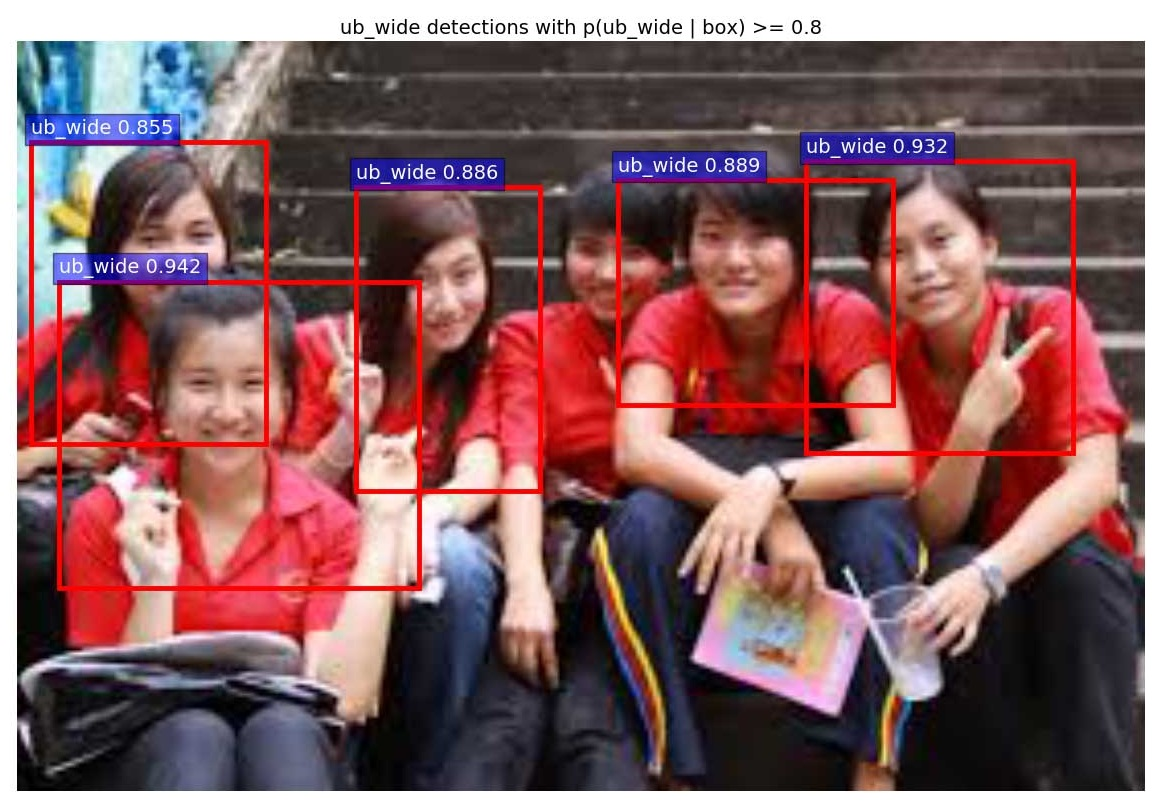
\includegraphics[width=60mm]{img2}} \label{fig:res2} &
%	\addheight{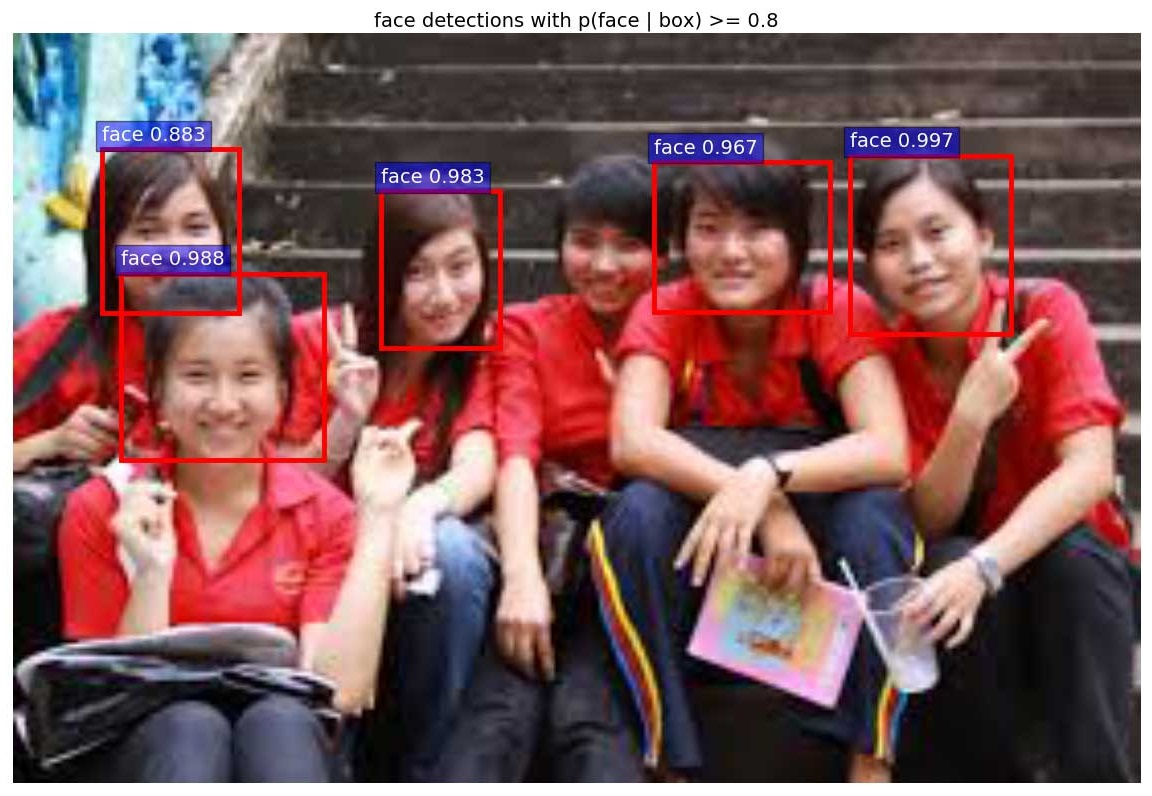
\includegraphics[width=60mm]{img3}} \label{fig:res3} &
%	\addheight{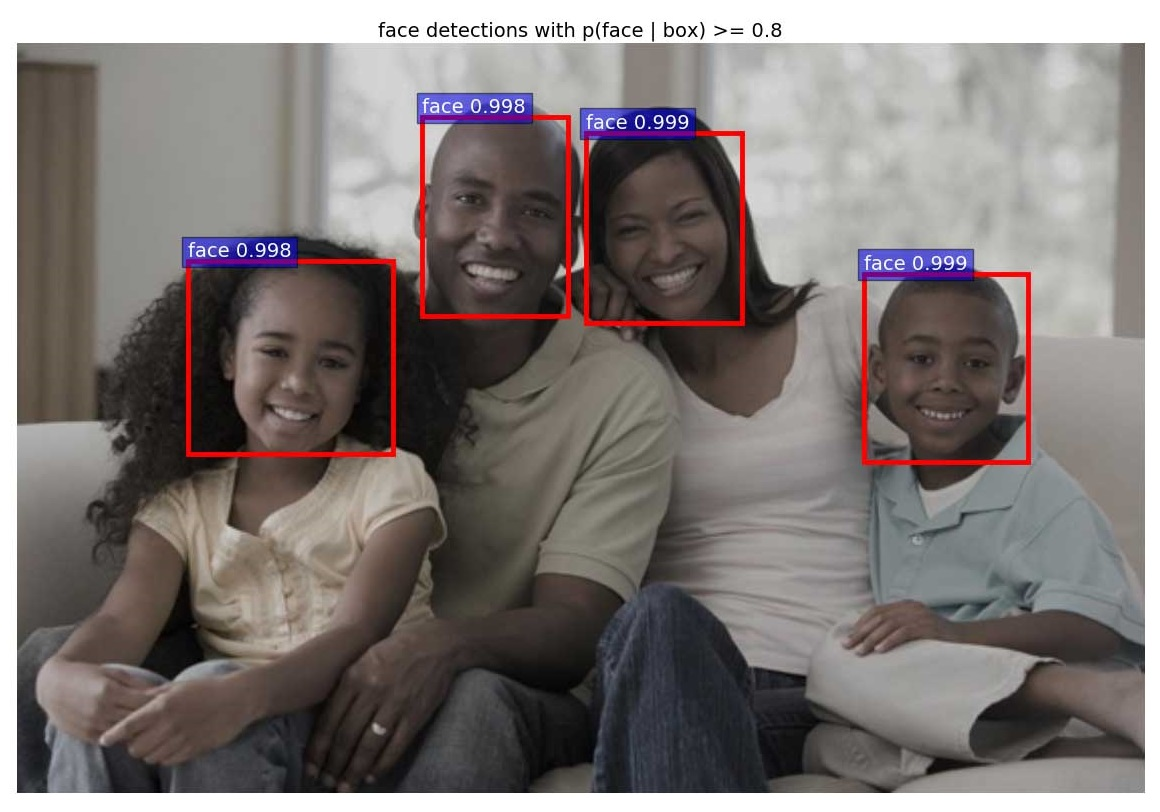
\includegraphics[width=60mm]{img4}} \label{fig:res4}	
%	\\
%	\small Result image 2 & Result image 3 &  Result image 4 \\
%	%\hline
%	\addheight{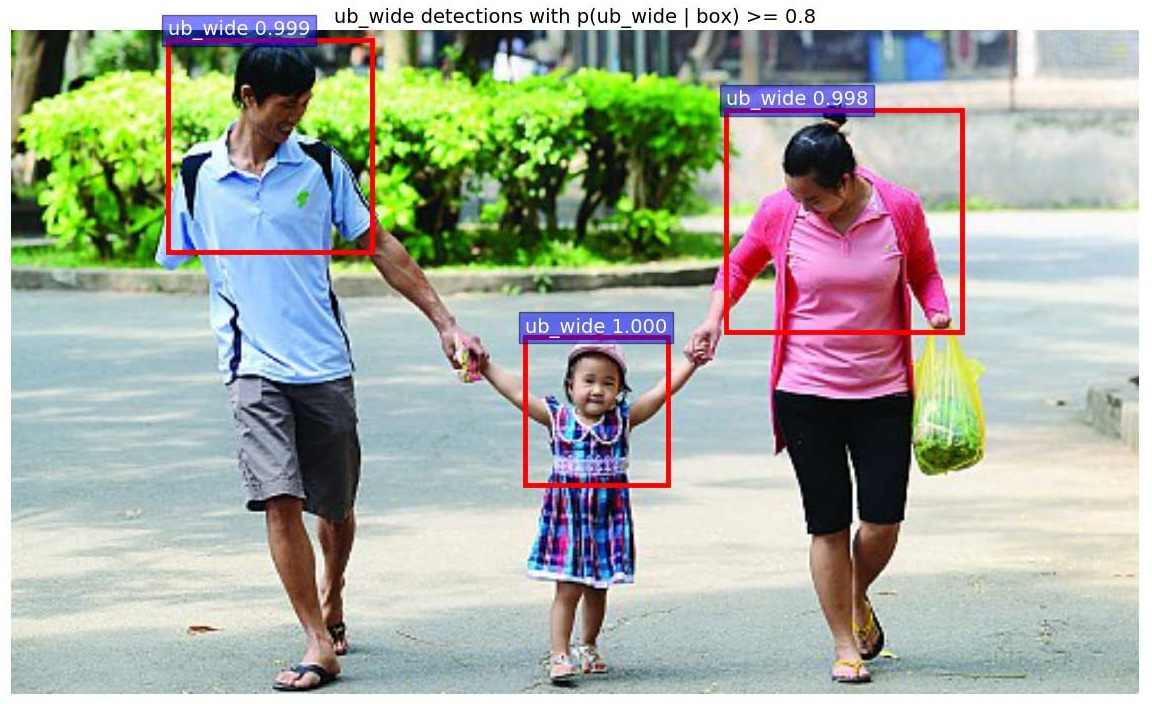
\includegraphics[width=60mm]{img5}} \label{fig:res5} &
%	\addheight{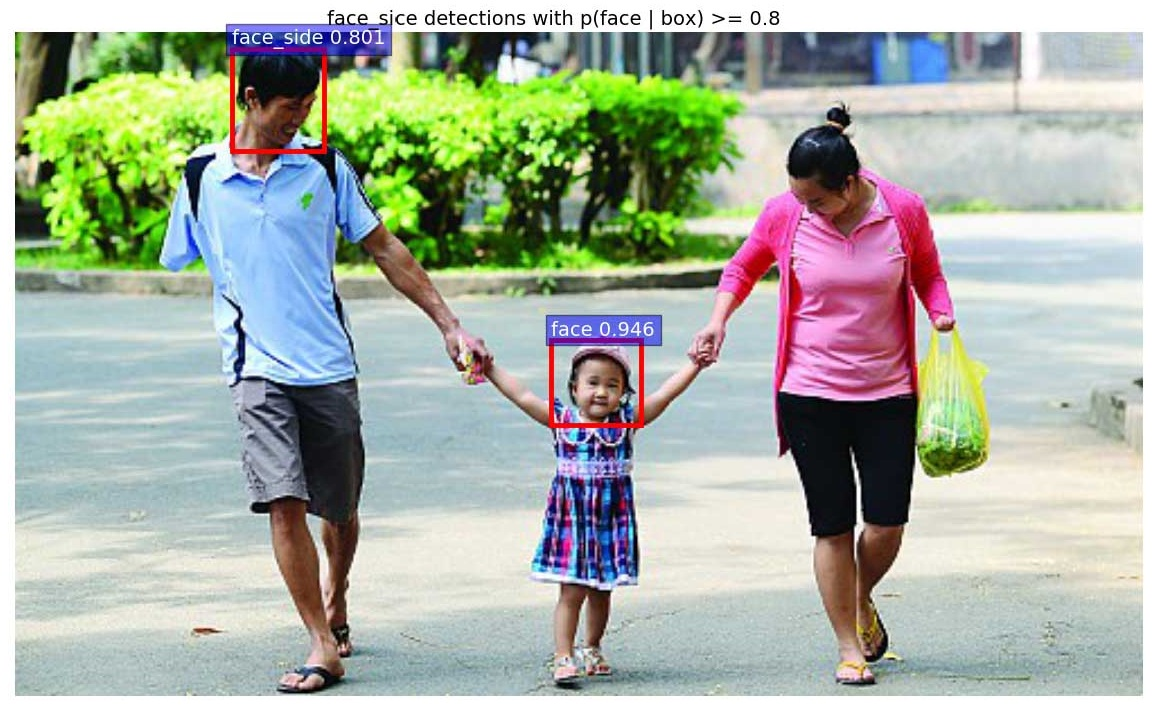
\includegraphics[width=60mm]{img6}} \label{fig:res6} &
%	\\
%	\small Result image 5 &  Result image 6 & \\
%	
%\end{tabular}
%\end{table*} 

In this test, the detector also found 5 faces, which are presented in \ref{fig:res3}. The undetected upper body's face is also undetected. This can be traced down to the limitation of the training stage, which only uses 98 images.

Still, this result is quit good, which gives R = 5/6 (about 83 \%)

In figure \ref{fig:res4}, all the upper bodies (and all faces) are detected with high certanties (\(> 0.95\)). This proves that in common cases, the detector can work well and give trusted result.
In this case, R = 1.

In figure \ref{fig:res5}, all upper bodies are detected correctly, which gives R = 1.

Only 2 out of 3 faces are detected. The last one is mostly obscured and too hard for the detector. \\
The average value of R = \(4/9 + 5/6 + 5/6 + 1 + 1) / 5 = 0.82\) \\
